\section{进程与线程}
\subsection{进程与线程}
\subsubsection{进程}
进程 (process) 是OS进行资源分配和调度的单位, 以特定形式存在于内存中, 具有一定的封闭性, 是多道技术的重要基础. 

\subsubsection{进程的状态与转换}
\begin{figure}[H]
    \centering
    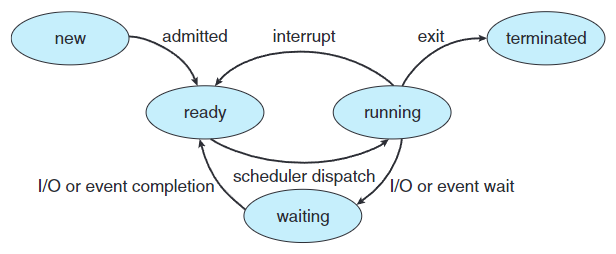
\includegraphics[width=0.88\linewidth]{pic/OS3/Diagram of process state}
    \caption{Diagram of process state}
\end{figure}

\subsubsection{进程的组成}
内核部分: 进程控制块(Process Control Block, PCB), 系统利用PCB来描述进程的基本情况和运行状态. 

用户部分: 
\begin{itemize}
    \item Text section: 存储代码
    \item Data section: 存储代码中的全局变量、静态变量;
    \item Heap section: 常说的“堆”, 被动态分配的内存;
    \item Stack section: 常说的“栈”, 存储一些暂时性的数据, 如函数传参、返回值、局部变量等;
\end{itemize}

\begin{figure}[H]
    \centering
    \begin{minipage}{0.48\linewidth}
        \centering
        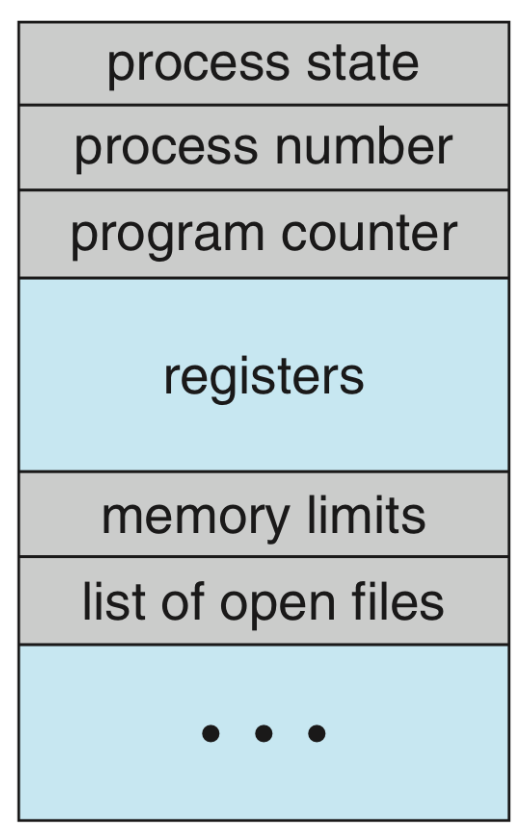
\includegraphics[height=\linewidth]{pic/OS3/PCB.png}
        \caption{PCB}
    \end{minipage}
    \begin{minipage}{0.48\linewidth}
        \centering
        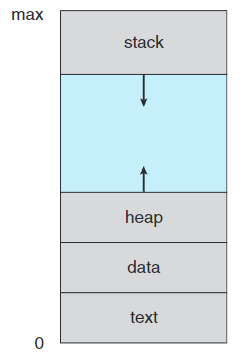
\includegraphics[height=\linewidth]{pic/OS3/Layout of a process in memory.png}
        \caption{Layout of a process in memory}
    \end{minipage}
    % \caption{}
\end{figure}

\subsubsection{进程控制}
\begin{enumerate}
    \item 进程的创建: fork() 创建进程, 该进程只有进程号与 parent 进程不一样, 同时通过检查返回值 pid 来判断属于 parent 还是 child. 
    \subitem 使用 execXX() 覆盖进程的地址空间, 以实现执行其他程序
    \item 进程的终止: exit() 终止进程, 同时返回状态值, 值被 parent 进程的 wait() 接收. 若 parent 没有 wait(), 进程变为僵尸进程, 被 systemd wait. 
    \item 进程的通信: 通过诸如 共享存储(shared memory), 消息传递(message passing), 文件 / 管道(pipe) 等 的方法通信
\end{enumerate}

\subsubsection{进程切换}
上下文切换(context switch): 切换CPU到另一个进程需要保存当前进程状态并恢复另一个进程的状态.

上下文可能包括: CPU 寄存器中的值, 进程状态, 内存的管理信息等. 
\begin{figure}[H]
    \centering
    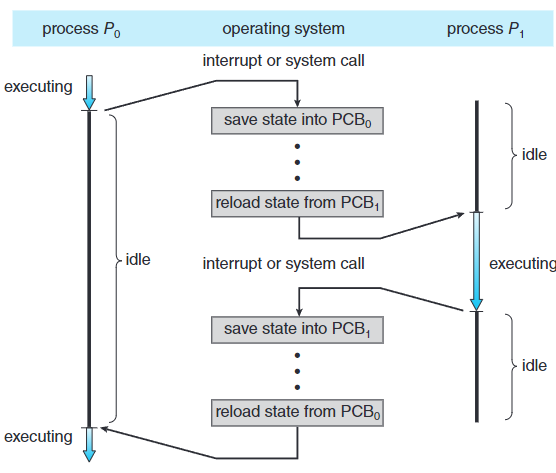
\includegraphics[width=0.618\linewidth]{pic/OS3/Diagram showing context switch from process to process}
    \caption{进程间的 context switch}
\end{figure}



\subsubsection{线程和多线程模型}
线程是一种轻量级的进程, 它在进程的基础上进行划分, 是进程内的一个可调度的执行单元, 以减小进程 folk 和切换的开销为目的. 

\begin{figure}[H]
    \centering
    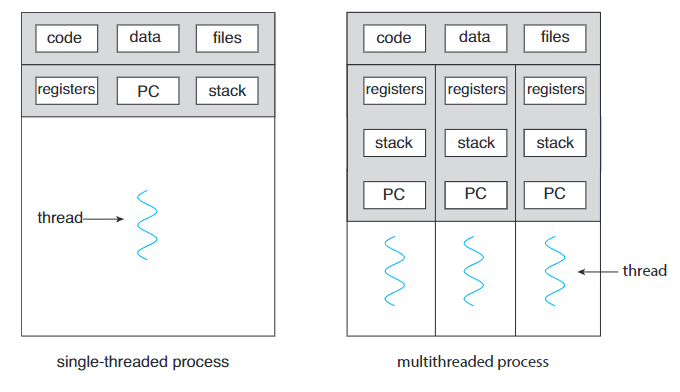
\includegraphics[width=0.618\linewidth]{pic/OS4/Single-threaded and multithreaded processes}
    \caption{Single-threaded and multithreaded processes}
\end{figure}

多线程模型, 由于用户级线程和内核级线程连接方式的不同, 分为三种. 

\begin{figure}[H]
    \centering
    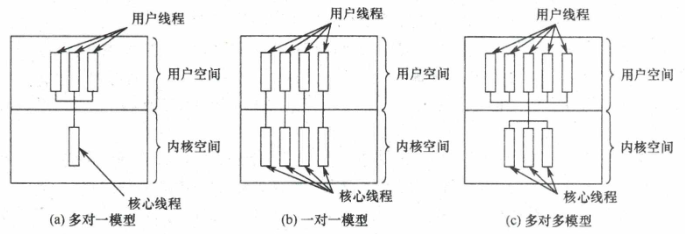
\includegraphics[width=0.88\linewidth]{pic/OS-CheatSheet/多线程模型.png}
    \caption{多线程模型}
\end{figure}

\subsection{进程调度}
调度问题(scheduling). 分为抢占式调度与非抢占式调度. 

\subsubsection{进程调度 Queues}
\begin{itemize}\small
    \item Job queue
    \subitem 系统中所有进程
    \item Ready queue
    \subitem 在 main memory 中的所有进程, 准备好等待运行
    \item Device queues
    \subitem 等待 I/O 设备的进程
\end{itemize}

\subsubsection{调度衡量标准}
\begin{itemize}\small
    \item CPU utilization (CPU利用率) 
    \subitem 应尽可能使CPU有效工作. 
    \item Throughput (吞吐率)
    \subitem 表示单位时间内CPU完成作业的数量. 
    \item Turnaround time (周转时间)
    \subitem 指从作业提交到作业完成所经历的时间. 
    \item Waiting time (等待时间)
    \subitem 指进程处于 \textbf{ready queue} 的时间之和(不算 I/O 时 的时间)
    \item Response time (响应时间)
    \subitem 指从用户提交请求到系统首次产生响应所用的时间.
\end{itemize}

\subsubsection{调度实现}
由 CPU scheduler 选择哪一个就绪态的将要被执行后, 由 dispatcher(调度器) 来完成具体的切换工作包括:
\begin{enumerate}
    \item 在两个进程间进行上下文切换;
    \item 切换到用户态;
    \item 跳转到用户程序中合适的位置以继续进程执行
\end{enumerate}
而从 dispatcher 停止上一个运行时的进程, 完成上下文切换, 并启动下一个进程的延时, 称为 dispatch latency. 

\subsubsection{调度算法}

\paragraph{FCFS} 是最基本的非抢占式调度方法, 就是按照进程先来后到的顺序进行调度. 

\paragraph{SJF}选择需要运行时间最短的进程先运行. 能够保证理论上平均等待时间最小; 但可能导致运行时间长的进程一直被推迟, 从而导致“饥饿”现象. 此外, 进程运行时间难以获知. 

\paragraph{Priority Scheduling}选择优先级最高的进程先运行. 可以分为抢占式或非抢占式实现. 可使用 priority aging, 让等待过久的任务赋予较高的优先级, 以此避免饥饿的发生. 

\paragraph{RR} 每一个进程最多连续执行一个时间片的长度, 完成后被插入到 FIFO ready queue 的末尾, 并取出 FIFO ready queue 的队首进行执行, 是使用分时技术后的 FCFS 调度. 若在时间片内进程完成运行可立即切换到下一个线程. 

\paragraph{Multilevel Queue}将 ready queue 分成多个队列, 每个队列使用不同的调度算法. 

\paragraph{Multilevel Feedback Queue}在 Multilevel Queue基础上, 允许进程在队列间转移, 以此实现更灵活更科学的调度

\subsection{同步与互斥}
\subsubsection{Background}
共享数据上的并发访问导致的不同步

\paragraph{Race Condition(竞态条件)}多个进程对寄存器中的内容进行并发的访问会发生竞态条件. 

\subsubsection{The Critical-Section Problem}
仅在 Critical section 中修改 register. 细粒度的 critical section 并发性更好. 

\begin{code}
    \begin{minted}{c++}
        do{
            Entry section;
            Critical section; // 临界区段
            Exit section;
            Remainder section;
        }while(TRUE);
    \end{minted}
    \caption{General structure of a typical process $P_j$}
\end{code}

Solution to Critical-Section Problem: 
\begin{enumerate}
    \item Mutual Exclusion (互斥): 对一个 critical section, 仅有一个相关进程可以运行. 
    \item Progress (空闲让进): 当无进程处于临界区, 可允许一个请求进入临界区的进程立即进入自己的临界区
    \item Bounded Waiting (有限等待): 对请求进入的进程, 保证能在有限时间内进入临界区. 
\end{enumerate}

\subsubsection{Peterson's Solution}
\begin{itemize}
    \item 只有两个进程参与
    \item 两个进程共享两个变量: 
    \begin{itemize}
        \item \mintinline{c++}{int turn} : 指示轮到谁进入临界区
        \item \mintinline{c++}{bool flag[2]} : 用于指示进程是否准备好进入临界区
    \end{itemize}
\end{itemize}

\begin{code}
    \centering
    \begin{minted}{c++}
        while (true) {
            flag[i] = TRUE;
            turn = j;
            while ( flag[j] && turn == j);
            CRITICAL SECTION;
            flag[i] = FALSE;
            REMAINDER SECTION;
        }
    \end{minted}
    \caption{The Algorithm for Process $P_i$}
\end{code}
但遇到指令重排会失效, 可在 \mintinline{c++}{flag[i]=TRUE}   后增加个内存屏障, 保证flag 都处理完才能进行下面的指令. 
\subsubsection{Synchronization Hardware}
在临界区关中断, 出了后再打开.

或使用一些 atomic 指令. 

\begin{code}
    \begin{minted}{c++}
        bool lock=false;

        bool TestAndSet (bool *target){
            bool rv = *target;
            *target = TRUE;
            return rv:
        }

        while (true) {
            while(TestAndSet(&lock))
                ; /* do nothing */
            critical section;
            lock = FALSE;
            remainder section;
        }
    \end{minted}
    \caption{TestAndSet}
\end{code}

\begin{code}
    \begin{minted}{c++}
        bool lock=false;

        void Swap (boolean *a, boolean *b){
            bool temp = *a;
            *a = *b;
            *b = temp:
        }

        while (true) {
            key = TRUE;
            while (key == TRUE)
                Swap (&lock, &key);
            critical section;
            lock = FALSE;
            remainder section;
        }
    \end{minted}
    \caption{Swap}
\end{code}

\subsubsection{Solution with Mutex Locks}
\begin{code}
    \begin{minted}{c++}
        void acquire(){
            while(!available)
                ; /* busy wait */
            available=false;
        }

        void release(){
            available=true;
        }
    \end{minted}
    \caption{acquire and release}
\end{code}
上述是自旋锁 (spin lock),  为 mutex lock 的一种实现, 其会存在忙等待 (busy waiting). 
\subsubsection{Semaphores(信号量)}
\begin{code}
    \begin{minted}{c++}
        struct Semaphore{
            int val;
            Semaphore(int _val)val(_val){}
        };

        void wait(Semaphore S){
            while(S.val<=0);
            S.val--;
        }

        void signal(Semaphore S){
            S.val++;
        }
    \end{minted}
    \caption{Semaphores with busy waiting}
\end{code}

\begin{code}
    \begin{minted}{c++}
        struct Semaphore{
            int val;
            struct process *L;
            Semaphore(int _val)val(_val){}
        };

        void wait(Semaphore S){
            S.val--;
            if(S.val<0){
                add this process to S.L;
                block(S.L);
            }
        }

        void signal(Semaphore S){
            S.val++;
            if(S.val<=0){
                remove a process P from S.L;
                wakeup(P);
            }
        }
    \end{minted}
    \caption{Semaphores without busy waiting}
\end{code}
signal 与 wait 都是 atomic 的. 

\begin{code}
    \begin{minted}{c++}
        Semaphore S(1); // initialized to 1
        wait(S);
        Critical Section;
        signal(S);
    \end{minted}
    \caption{Semaphore Usage}
\end{code}

\subsubsection{Monitors(管程)}
管程定义了一个数据结构和能为并发进程所执行(在该数据结构上)的一组操作, 这组操作能同步进程和改变管程中的数据. 管程中一次只能有一个进程处于活动状态. 

\paragraph{条件变量(Condition Variables)}将进程阻塞原因定义为条件变量. 对条件变量只能进行两种操作, 
\begin{itemize}\small
    \item x.wait:当x对应的条件不满足时, 正在调用管程的进程调用x.wait将自己插入x条件的等
    待队列, 并释放管程. 此时其他进程可以使用该管程. 
    \item x.signal: x对应的条件发生了变化, 则调用x.signal,唤醒一个因x条件而阻塞的进程. 
\end{itemize}

% 经典题 记了也不会考, 不记了
% 做了一会, 发现经典题不愧是经典题, 还是记一记吧 
\subsubsection{同步问题例子}
\paragraph{缓存有界}缓存区存在上界, 使用 empty 与 full两个信号量控制缓存区, 缓存区是否需要再一个信号保护依据题目决定. 

例如, 缓存区至多缓存 $N$个物品, $A$ 生成物品放入缓存区, $B$ 从缓存区中取出消耗物品
\begin{minted}{c++}
    Semaphore empty=N, full=0, mutex=1;
\end{minted}
\vspace{-\medskipamount}
\vspace{-2\baselineskip}
\vspace{0.4pt}
\begin{multicols}{2}
    \begin{minted}{c++}
        A{
            P(empty);
            P(mutex);
            product;
            V(mutex);
            V(full);
        }
    \end{minted}
    \columnbreak
    \begin{minted}{c++}
        B{
            P(full);
            P(mutex);
            consume;
            V(mutex);
            V(empty);
        }
    \end{minted}
\end{multicols}

\paragraph{同类并发}设定count计数, 并在为0时作特殊处理. 记得 count 需要保护. 

例如, 有 $A, B$ 两种进程需要一项资源$s$, 但多个$A$或多个$B$可以同时使用.
\begin{minted}{c++}
    Semaphore s=1, sa=1, sb=1;
    int counta=0, countb=0;
\end{minted}
\vspace{-\medskipamount}
\vspace{-2\baselineskip}
\vspace{0.4pt}
\begin{multicols}{2}
    \begin{minted}{c++}
        A{
            P(sa);
            if(counta==0)P(s);
            counta++;
            V(sa);
            run A;
            P(sa);
            counta--;
            if(counta==0)V(s);
            V(sa);
        }
    \end{minted}
    \columnbreak
    \begin{minted}{c++}
        B{
            P(sb);
            if(countb==0)P(s);
            countb++;
            V(sb);
            run A;
            P(sb);
            countb--;
            if(countb==0)V(s);
            V(sb);
        }
    \end{minted}
\end{multicols}


\paragraph{依赖关系}为所依赖的资源设定 信号量. 

例如, $T_1: A, C,\ T_2: B$, 运行顺序为 $A\to B\to C$. 
\begin{minted}{c++}
    Semaphore A=0,B=0;
\end{minted}
\vspace{-\medskipamount}
\vspace{-2\baselineskip}
\vspace{0.4pt}

\begin{multicols}{2}
    \begin{minted}{c++}
        T1{       
            run A;
            V(A); 
            P(B); 
            run C;
        }
    \end{minted}
    \columnbreak
    \begin{minted}{c++}
        T2{
            P(A);
            run B;
            V(B);
        }
    \end{minted}
\end{multicols}


\subsection{Deadlocks}
\subsubsection{概念}
Deadlocks指多个进程因竞争资源而造成的互相等待. 


但同时满足以下四个条件时, 死锁产生. 
\begin{enumerate}
    \item Mutual exclusion(互斥性): 一个 resource 只能同时被一个 process 使用. 
    \item Hold and wait: 进程手里至少有一个 resource, 且等待其他进程的 resource. 
    \item No preemption: 不能抢占
    \item Circular wait: 循环等待. 
\end{enumerate}

\subsubsection{预防}
防止死锁的发生只需破坏死锁产生的4个必要条件之一即可. 
\begin{enumerate}
    \item Mutual Exclusion: 难以打破. 
    \item Hold and Wait: 让一个线程/进程一旦申请资源就一次性获取所有资源, 如果没法一次性获取所有资源就释放已经申请到的资源
    \item No Preemption: 也不太行
    \item Circular Wait: 通过给资源编号, 规定进程/线程只能按特定的顺序申请资源 (但难以做到)
\end{enumerate}
\subsubsection{避免}
\paragraph{资源分配图}是一种有两类节点的有向图, 我们用圆节点 $T_i$ 表示进程/线程, 用方节点 $R_j$ 表示资源, 方节点中的实心点表示一个资源类别的一个实例. 

\begin{figure}[H]
    \centering
    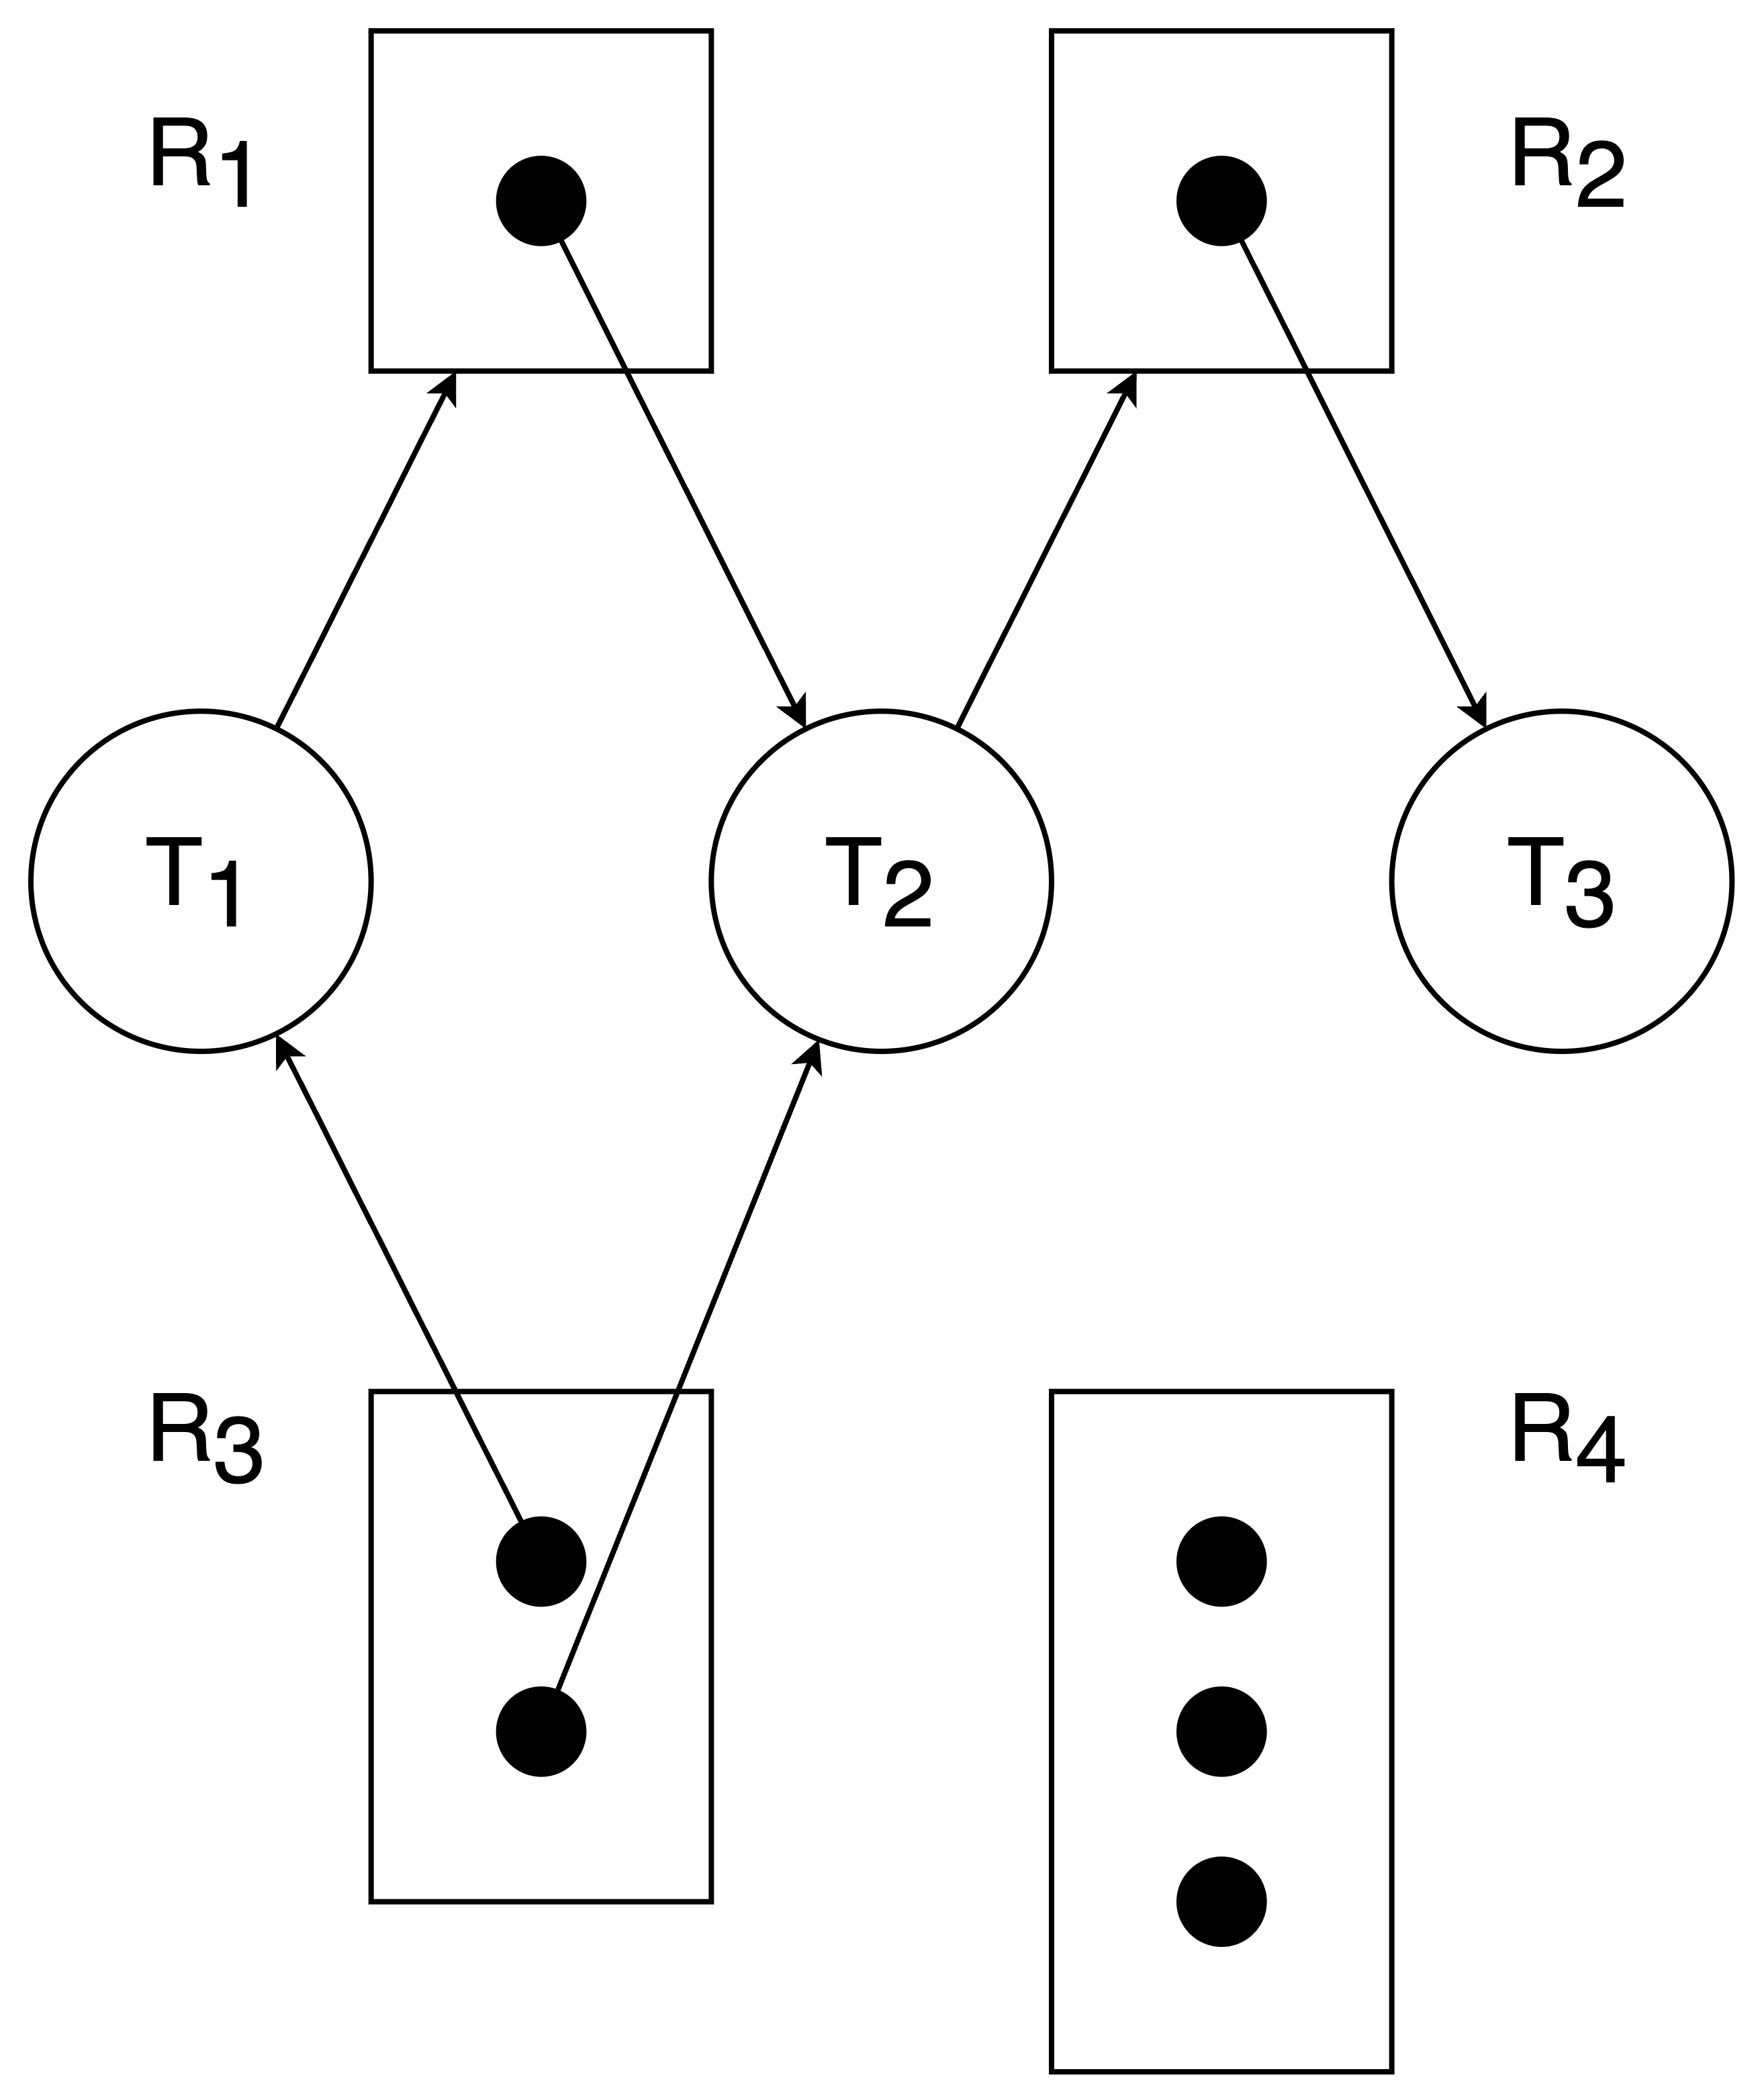
\includegraphics[width=0.22\linewidth]{pic/OS-CheatSheet/资源分配图}
    \caption{资源分配图}
\end{figure}

\paragraph{银行家算法}就是需要动态地检测某个资源申请是否会导致系统进入不安全状态, 如果会导致系统进入不安全状态, 则等待资源足够再分配. 

数据结构:
\begin{itemize}
    \item $Available$(可利用资源向量) $M$
    \item $Max$(最大需求矩阵) $N\times M$
    \item $Allocation$(分配矩阵) $N\times M$
    \item $Need$(需求矩阵) $N\times M$
\end{itemize}
\begin{align*}
    Need = Max-Allocation
\end{align*}

\begin{algorithm}[H]
    \caption{银行家算法}
    \begin{algorithmic}
        \Require $Request_i\ M$, 表示进程 $P_i$ 请求资源的数量
        \If{$Request_i\le Need_i$ and $Request_i\le Available_i$}
            \State 系统尝试分配资源:
            \begin{align*}
                Available&-=Request\\
                Allocation_i&+=Request\\
                Need_i&-=Request
            \end{align*}
            \State 运行安全性算法检查分配后是否处于安全状态
            \If{安全}
                \State 完成分配
            \Else
                \State 恢复分配, 并让$P_i$继续等待
            \EndIf
        \Else
            \State 无法或无需分配
        \EndIf
    \end{algorithmic}
\end{algorithm}

\begin{algorithm}[H]
    \caption{安全性算法}
    \begin{algorithmic}
        \State 初始化安全序列, $Work=Available$, 表示当前状态的剩余资源量
        \While{寻找 $i$, 有 $i$不在安全序列并且 $Need_i\le Work$}
            \State 把 $i$ 加入安全序列
            \State $Work+=Allocation_i$
        \EndWhile
        \State 若安全序列有所有进程, 则系统安全, 否则不安全. 
    \end{algorithmic}
\end{algorithm}

\subsubsection{检测}

\paragraph{面向单实例资源检测}反正就是资源状态图


\subsubsection{解除}
\begin{enumerate}
    \item 都别活, 杀死所有死锁中的进程/线程
    \item 一个一个杀, 杀到没有死锁
    \item 留活命, 但是需要回滚部分进程, 强行抢占占有的资源
\end{enumerate}